\documentclass[12pt]{article}
\usepackage{amsmath}
\usepackage{enumerate}
\usepackage{mathrsfs} 
\usepackage{amsthm}
\usepackage{amsfonts}
\usepackage{amssymb}
\usepackage{latexsym} 
%\usepackage{epsfig}
%\usepackage{graphicx}
%\usepackage[dvips]{graphicx}
\usepackage{tikz}
\usepackage{tikz-cd}



\usepackage[matrix,tips,graph,curve]{xy}

\newcommand{\mnote}[1]{${}^*$\marginpar{\footnotesize ${}^*$#1}}
\linespread{1.065}

\makeatletter

\setlength\@tempdima  {5.5in}
\addtolength\@tempdima {-\textwidth}
\addtolength\hoffset{-0.5\@tempdima}
\setlength{\textwidth}{5.5in}
\setlength{\textheight}{8.75in}
\addtolength\voffset{-0.625in}

\makeatother

\makeatletter 
\@addtoreset{equation}{section}
\makeatother


\renewcommand{\theequation}{\thesection.\arabic{equation}}

\theoremstyle{plain}
\newtheorem{theorem}[equation]{Theorem}
\newtheorem{corollary}[equation]{Corollary}
\newtheorem{lemma}[equation]{Lemma}
\newtheorem{proposition}[equation]{Proposition}
\theoremstyle{definition}
\newtheorem{definition}[equation]{Definition}
\newtheorem{definitions}[equation]{Definitions}
%\theoremstyle{remark}

\newtheorem{remark}[equation]{Remark}
\newtheorem{remarks}[equation]{Remarks}
\newtheorem{exercise}[equation]{Exercise}
\newtheorem{example}[equation]{Example}
\newtheorem{examples}[equation]{Examples}
\newtheorem{notation}[equation]{Notation}
\newtheorem{question}[equation]{Question}
\newtheorem{assumption}[equation]{Assumption}
\newtheorem*{claim}{Claim}
\newtheorem{answer}[equation]{Answer}
%%%%%% letters %%%%

\newcommand{\fa}{\mathfrak{a}}
\newcommand{\fb}{\mathfrak{b}}
\newcommand{\fm}{\mathfrak{m}}
\newcommand{\fp}{\mathfrak{p}}
\newcommand{\fq}{\mathfrak{q}}
\newcommand{\sP}{\mathcal{P}}

\newcommand{\IA}{\mathbb{A}}
\newcommand{\IN}{\mathbb{N}}
\newcommand{\IF}{\mathbb{F}}
\newcommand{\IP}{\mathbb{P}}
\newcommand{\IZ}{\mathbb{Z}}

\newcommand{\sO}{\mathcal{O}}

\newcommand{\shF}{\mathscr{F}}
\newcommand{\shG}{\mathscr{G}}
%%%%%%% macros %%%%%

%% my definitions %%%

\newcommand{\End}{\mathrm{End}}
\newcommand{\tr}{\mathrm{tr}}
\newcommand{\Hom}{\mathrm{Hom}}
\newcommand{\Aut}{\mathrm{Aut}}
\newcommand{\Trace}{\mathrm{Trace}\,}
\newcommand{\rank}{\mathrm{rank}}
\renewcommand{\deg}{\mathrm{deg}\,}
\newcommand{\Spec}{\rm Spec\,}
\newcommand{\Sym}{\mathrm{Sym \,}}
\newcommand{\Span}{\mathrm{Span \,}}
\renewcommand\dim{{\rm dim\,}}
\renewcommand\det{{\rm det\,}}
\newcommand{\sing}{{\rm sing}}


\newcommand\iso{{\, \cong \,}} 
\newcommand\tensor{{\otimes}}
\newcommand\Tensor{{\bigotimes}} 
\newcommand\union{\bigcup} 
\newcommand\onehalf{\frac{1}{2}}
\newcommand\trivial{{\mathbb I}}
\newcommand\wb{\overline}

%%%%%Delimiters%%%%

\newcommand{\<}{\langle}
\renewcommand{\>}{\rangle}

%\renewcommand{\(}{\left(}
%\renewcommand{\)}{\right)}


%%%% Different kind of derivatives %%%%%

\newcommand{\delbar}{\bar{\partial}}
\newcommand{\pdu}{\frac{\partial}{\partial u}}
%\newcommand{\pd}[1][2]{\frac{\partial #1}{\partial #2}}
\newcommand{\fl}[1]{\lfloor #1 \rfloor}

%%%%% Arrows %%%%%
\newcommand{\induce}{\rightsquigarrow}
\newcommand{\into}{\hookrightarrow}
\newcommand{\onto}{doubleheadarrow}
\newcommand{\tto}{\longmapsto}
\def\llra{\longleftrightarrow}
\def\wt{\widetilde}
\def\wtilde{\widetilde}
\def\what{\widehat}
\def\bf{\textbf}
\def\it{\textit}
%%%%%%%%%%%%%%%%%%% Ziquan's definitions %%%%%%%%%%%%%%%%%%%%
\newcommand{\Ann}{\mathrm{Ann}}
\newcommand{\height}{\mathrm{height \,}}
\newcommand{\Div}{\mathrm{Div}}
\newcommand{\sE}{\mathcal{E}}
\newcommand{\sQ}{\mathcal{Q}}
\newcommand{\p}{\partial}
\newcommand{\im}{\mathrm{im}\,}
\newcommand{\grad}{\mathrm{grad}\,}
\newcommand{\proj}{\mathrm{proj}}
\newcommand{\Prob}{\mathrm{Prob}}
%%%%%%%%%%%%% new definitions for the positive mass paper %%%%%%%%%

\newcommand{\sperp}{{\scriptscriptstyle \perp}}
\newcommand{\st}{\mathrm{s.t.}\,}

%%%%%%%%%%%%%%%%%%%%%%%

%%%%%%%%%%%%%%%%%%%%%%%%%%%%%%%%%%%%%%%%%%%%%



%
\begin{document}
%

\title{A Bertini Existence Theorem on Elliptic Surfaces}
\author{Ziquan Yang}


\date{August 14, 2015}

\maketitle
 
%\setcounter{secnumdepth}{1} 

\setcounter{section}{0}

\section{Introduction}
Consider hypersurfaces in $\IP^2 \times \IP^1$ of bidegree $(3, d)$ over some base field $k$. These hypersurfaces are parametrized by $P = \IP V$, where
$$ V = H^0 ( \IP^2 \times \IP^1, \sO(3, d) ) $$
Let $P^0$ be the subscheme parametrizing those non-singular ones:
$$ P^0 = \{ f \in P : H_f \textit{ is non-singular }\} $$
Let $\pi : \IP^2 \times \IP^1 \to \IP^1$ be projection to the second component. If $H_f$ is non-singular, then fibers of $\pi|_{H_f}$ are cubic curves in $\IP^2$. This makes $H_f$ an elliptic surface. The analogy of being simply ramified for $H_f$ has to do with singular fibers of the map $\pi : H_f \to \IP^1$. Smooth fibers are all isomorphic to the smooth cubic curve. It is customary for some literature to call an irredcucible cubic curve, together with a specified point as the base point, an elliptic curve. There are many types of singular fibers. If the fiber is irreducible, then it is either a nodal curve (e.g. $y^2 = x^2 - x^3$), or a cuspidal curve (e.g. $y^2 = x^3$). If the fiber is not irreducible, then it may be a union of a conic curve and a line, or a union of three lines and there are many different configurations of irreducible components. 
An analogue of a simply ramified curve would be a hypersurface whose singular fibers are all nodal curves. Why is an analogue would be clear in the discussion of Euler characteristics. Hence we are primarily concerned with the following subset of $P^0$: 
$$ D = \{ f \in P^0 : \textit{all singular fibers of $H_f$ are nodal curves} \}$$

For future use we introduce some notation. Let $X$ be a scheme and $f : X \to Y$ be a morphism. For $P \in Y$, we denote the fiber $f^{-1}(P)$ by $X_P$ when $f$ is clear in the context. We denote the singular locus of $X$ by $X_\sing$. 

\section{Euler Characteristic}
Just like the genus of a curve tells us the degree of the ramification divisor for a curve of bidegree $(n, d)$ in $\IP^1 \times \IP^1$, the Euler characteristic of a hypersurface in $\IP^2 \times \IP^1$ tells us something about singular fibers. Let $f \in P^0$ and $H_f$ be the corresponding hypersurface. With respect to the map $\pi : H_f \to \IP^1$ we may write $X$ as $X^0 \coprod C$, where $C$ is the finite set of points with singular fibers and $X^0$ is its complement, and $Y$ as $Y^0 \coprod \pi^{-1}(C)$, where $Y^0 = \pi^{-1} X^0$. Let $F$ be the smooth cubic curve in $\IP^2$, we see that $Y^0$ is a $F$-bundle of $X^0$, and their Euler characteristics are related by 
$$ e(Y^0) = e(X^0 ) \cdot e(F) $$ 
Since $e(F) = 0$ we have that $e(Y^0) = 0$. Now since $Y = Y^0 \coprod \pi^{-1}(C)$, we see that $e(Y) = e(Y^0) + e(\pi^{-1}(C)) = e(\pi^{-1}(C))$. Note that $C$ is a finite set of points, and hence $\pi^{-1} (C)$ is a disjoint union of singular cubic curves. 

\begin{figure}[h!]
  \centering
      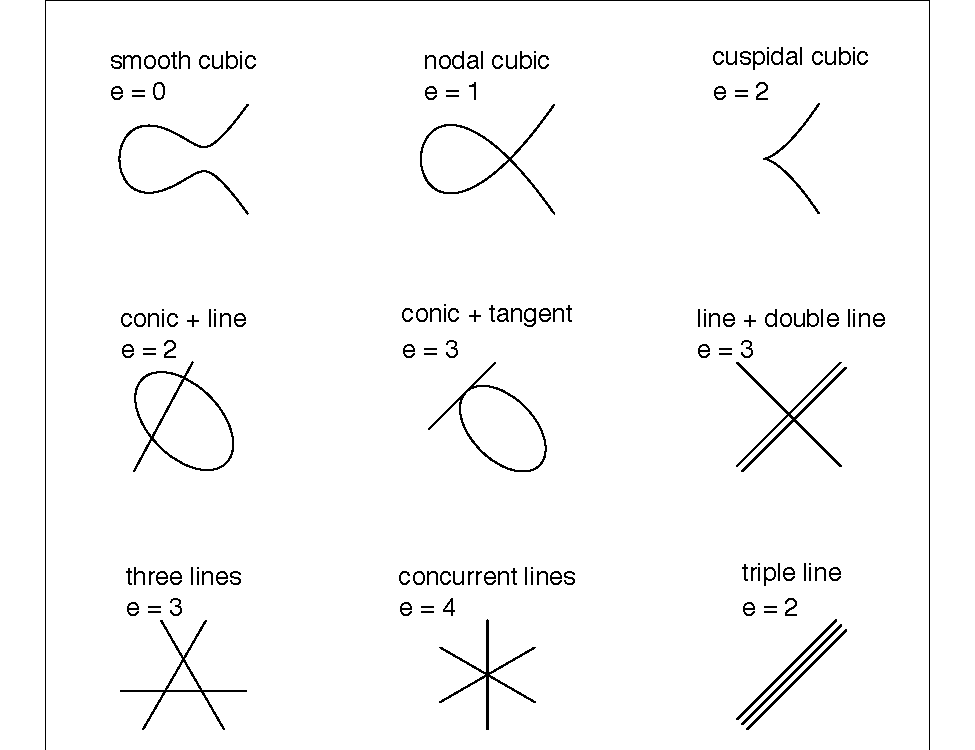
\includegraphics[width=1.0\textwidth]{planecubics}
  \caption{Cubic plane curves and their Euler characteristics \cite{Pic}}
\end{figure}
From the table we see that if $f \in D$, then $e(H_f)$ is exactly the number of points in $\IP^1$ over which the fibers are singular. In this sense, these hypersurfaces are analogues of simply ramified curves in $\IP^1 \times \IP^1$. 

Now we compute $e(H_f)$. In fact we do a more general computation, since it is not harder. Let $H_f \subseteq \IP^2 \times \IP^1$ be a smooth hypersurface of bidegree $(n, d)$. We denote the projections of $\IP^2 \times \IP^1$ onto the first and second components by $\pi_1, \pi_2$ respectively. Let $H_1$ be a hyperplane of $\IP^2$ and $H_2$ be a hyperplane of $\IP^1$. We think of them as generators of the Chow groups of their respective projective schemes. We define 
$$ A = \pi_1^*(H_1), \, E = \pi_2^*(H_2) $$
and $$ h_1 = A \cap H_f, \, h_2 = E \cap H_f $$
We compute the Chern classes of $H_f$ using the standard exact sequence:
$$ 0 \to T_{H_f} \to T_{\IP^2 \times \IP^1|_{H_f}} \to N_{H_f/\IP^2 \times \IP^1} \to 0$$
By Whitney\rq{}s formula, their total Chern classes are related by
$$ c(T_{\IP^2 \times \IP^1|_{H_f}}) = c(T_{H_f}) c(N_{H_f/\IP^2 \times \IP^1}) $$
Now $T_{\IP^2 \times \IP^1|_{H_f}}$ is $T_{\IP^2 \times \IP^1} = \pi_1^* T_{\IP^2} \oplus \pi_2^* T_{\IP^1}$ restricted to $H_f$, so we obtain 
$$ c(T_{\IP^2 \times \IP^1|_{H_f}}) = (1 + 3h_1 + 3h_1^2)(1 + 2h_2) $$
If $\iota : H_f \into \IP^2 \times \IP^1$ is the inclusion, then $$N_{H_f/\IP^2 \times \IP^1} = \iota^* \sO_{\IP^2 \times \IP^1}(nA  + dE) = (1 + nh_1 + dh_2)$$
Therefore 
\begin{align*}
c(T_{H_f}) &= c(T_{\IP^2 \times \IP^1|_{H_f}})c(N_{H_f/\IP^2 \times \IP^1})^{-1}\\
&= (1 + 3h_1 + 3h_1^2)(1 + 2h_2)(1 + nh_1 + dh_2)^{-1}\\
&= (1 + 3h_1 + 3h_1^2)(1 + 2h_2)(1 - (nh_1 + dh_2) + (nh_1 + dh_2)^2 - \cdots)
\end{align*}
In particular we obtain 
$$ c_2(T_{H_f}) = (n^2 - 3n + 3)h_1^2 + (6 + 2nd - 2n - 3d)h_1 h_2 $$
which is the top Chern class. Now we compute 
\begin{align*}
\deg h_1^2 &= A \cdot A \cdot (nA + dE) = d \\
\deg h_1 h_2 &= A \cdot E \cdot (nA + dE) = n 
\end{align*}
Finally we obtain 
$$ e(H_f) = \deg c_2(T_{H_f}) = 6n + 3d + 3n^2 d - 6 dn - 2n^2 $$
In particular, for future use we want to fix $n = 3$, so $e(H_f)$ depends only on $d$. In this case $e(H_f) = 12 d$.  

\section{An Analogue of Bertini\rq{}s Theorem}
We show an analogue of Bertini's theorem: 
\begin{theorem}
\label{Bertini}
Let the base field $k$ be algebraically closed. Let $V, P^0$ and $D$ be defined as before. Then for each $d$, $D$ is a constructible subset of $\IP V$, and $D \neq \IP V$. 
\end{theorem}

Let us consider $f$ on an affine chart $\IA^2 \times \IA^1$. Let its coordinates by $((x, y), t)$. $f$ can be written as
$$ f = \sum_{0 \le i + j \le 3} \sum_{0 \le k \le d} a_{ijk} x^i y^j t^k $$ and let 
$$ f_{ij} = \sum_{0 \le k \le d} a_{ijk} t^k $$
Fix $t_0 \in \IA$ and consider $f_{t_0} = \sum f_{ij}(t_0) x^i y^j$. $\deg f_{t_0} \le 3$ and $\{f_{t_0} = 0 \}$ described a curve $C_{f_{t_0}}$ in $\IA^2$. We may decompose $f_{t_0}$ into homogeneous components:
$$ f_{t_0} = f_{t_0, 0} + f_{t_0, 1} + f_{t_0, 2} + f_{t_0, 3} $$
Let us take $(0, 0)$ as an example to illustrate the observations. If $f_{t_0, 0} = f_{t_0, 1} = 0$, then the curve $C_{f_{t_0}}$ has a singularity at $(0, 0)$. 

\begin{enumerate}
\item If in addition $f_{t_0, 2} = 0$, then for sure $f_{t_0, 3}$, hence $f_{t_0}$ will factor and hence $C_{f_{t_0}}$ contains a line through $(0, 0)$. $C_{f_{t_0}}$ might be concurrent lines or a triple line, or a line + a double line. 

\item If $f_{t_0, 2} \neq 0$ but as a homogeneous polynomial of degree it vanishes twice at a point in $\IP^1$, then the tangent cone of $C_{f_{t_0}}$ contains a double line. $C_{f_{t_0}}$ might be a cusp, or a conic + a tangent. 

\item If $f_{t_0, 2} \neq 0$ and has two distinct roots in $\IP^1$, but it shares a least one root with $f_{t_0, 3}$, then the tangent cone of $C_{f_{t_0}}$ at $(0, 0)$ contains two lines, and one of the lines is an irreducible component of $C_{f_{t_0}}$. $C_{f_{t_0}}$ might be a conic plus a line (not tangent to it), or three lines. 

\item If $f_{t_0, 2} \neq 0$, has two distinct roots in $\IP^1$, and does not have a common root with $f_{t_0, 3}$ in $\IP^1$, then it must be a nodal curve. 
\end{enumerate}
In general, for each $t_0$ we can shift any point $(x_0, y_0)$ to the origin using Taylor expansion.
The above discussion naturally leads us to consider the scheme $\IP^1 \times \IA^2 \times \IA^1 \times \IP V$. We write its coordinates as $((u : v), (x, y), t, f)$. We want a subscheme $G$ to parametrize those tuples such that $f_t$ is singular at $(x, y)$, and in addition either $f_{t, 2}$ has a double root at $(u : v)$, or $f_{t, 2}(u : v) = f_{t, 3}(u : v) = 0$. The image of $G$ under the projection to $\IP V$ contains those hypersufaces that contain singular fibers other than a nodal curve. Conversely, these hypersurfaces lie in the image of some $G$ corresponding to the affine chart $\IA^2 \times \IA^1$. Since $X$ is covered by finitely many $\IA^2 \times \IA^1$, we reduce to studying one such $G$. 

We define $T^k_{(x_0, y_0)}f_{t_0} (u, v), 0 \le k \le 3$ to be terms in the Taylor expansion of $f_{t_0}$ at $(x_0, y_0)$:
$$ T^k_{(x_0, y_0)}f_{t_0} (u, v) = \sum_{0 \le i \le k} {k \choose i} \frac{\p^k f}{\p x^i \p y^j}(x_0, y_0) u^i v^{k - i} $$
and hence
$$ f_{t_0}(x, y) = \sum_{k = 0}^3 \frac{1}{k!} T^k_{(x_0, y_0)}f_{t_0}(x - x_0, y - y_0) $$
Let $G_s \subseteq \IP^1 \times \IA^2 \times \IA^1 \times \IP V$ be described by the following $3$ conditions:
\begin{align*}
f_t(x , y) = 0 ; 
\frac{\p f_t}{\p x} (x, y) = 0 ; 
\frac{\p f_t}{\p y} (x, y) = 0 
\end{align*}
Note that $G_s$ is independent of $(u : v)$. Now define $G_1 \subseteq G_s$ by appending two more conditions:
\begin{align*}
T^2_{(x, y)}f_{t} (u, v) &= 0 \\
T^3_{(x, y)}f_{t} (u, v) &= 0 
\end{align*}
and define $G_2 \subseteq G_s$ by appending the condition 
$$ T^2_{(x_0, y_0)}f_{t_0} \text{ has a double root at } (u : v) $$
For each $(u : v)$ the above amounts to two linear conditions on $T^2_{(x_0, y_0)}f_{t_0}$. 
We have that $G = G_1 \cup G_2$. 
At each point $((u : v), (x, y), t)$, condition that $((u : v), (x, y), t, f) \in G$ amounts to 5 linear conditions on coefficients of $f$.

\section{A Density Result}
Now we deal with the case when the base field $k$ is a finite field $\IF_q$. Let $p = \mathrm{char}\, \IF_q$ and we assume $p \neq 2, 3$. 
Let $R_{3, d} = H^0(\IP^2 \times \IP^1, \sO(3, d))$. If $S \subseteq \union_d R_{3, d}$, we say the probability of $f \in S$ as $d \to \infty$ is:
$$ \Prob(f \in S) = \lim_{d \to \infty} Prob(f_d \in S \cap R_{3, d}) = \lim_{d \to \infty} \frac{|S \cap R_{3, d}|}{|R_{3, d}|} $$
Let $D \subseteq \union_d R_{3, d}$ be the subset consisting of those $f$ such that $H_f$ is a smooth hypersurface in $\IP^2 \times \IP^1$ and has no singular fibers over $\IP^1$ other than nodal curves. 
\begin{theorem}
$ \Prob(f \in D) > 0 $ and hence when $d$ is sufficiently large, there always exists some smooth hypersurface of bidegree $(3, d)$, singular fibers of which are all nodal curves. 
\end{theorem}


We will follow the basic idea of the proof of Theorem~\ref{Bertini} so will use the same notations as before. 
\subsection{Lemmas}
Let $P \in \IP^1_{\IF_q}$ be a point. We say that a hypersuface $H_f$, or sometimes the polynomial $f \in H^0(\IP^2 \times \IP^1, \sO(3, d))$ defining it, is \textit{good} at the point $P$ if $H_f$ is smooth at all points $Q \in \pi^{-1}(P)$, and the fiber $(H_f)_P \subseteq \IP^2_{\kappa(P)}$ is either smooth or a nodal curve. Otherwise, we say $H_f$, or $f$, is \textit{bad} at $P$.  

Consider the vector space $H^0(\IP^2_{\IF_{q^e}}, \sO(3))^2$, we say that a pair $(F_1, F_2)$ is good if, it satisfies one the following conditions:
\begin{enumerate}
\item $F_1$ describes a smooth curve in $\IP_{\IF_{q^e}}$.
\item $F_1$ describes a nodal curve but $F_2$ does not vanish at the node.
\end{enumerate}  

\begin{lemma}
Let $P \in \IP^1$ be a fixed point and let $e = \deg P$. Let $r(s) \in \IF_q[s]$ be an irreducible polynomial such that the second infinitestimal neighborhood $P^{(2)} = \Spec \IF_q[s]/r(s)^2$. Let $\, \wt{} : \IF_q[s]/r(s) \to \IF_q[s]/r(s)^2$ be a section of the reduction map $\, \bar{} : \IF_q[s]/r(s)^2 \to \IF_q[s]/r(s)$. Then the map
$$ \varphi : H^0(\IP^2_{q^e} , \sO(3))^2 \to H^0(\IP^2_{q^e} \times P^{(2)}, \sO(3))$$ defined by 
$$ (F_1, F_2) \mapsto \wt{F_1} + r(s) F_2 $$
is an isomorphism of vector spaces. Moveover, $f$ is good at $P$ if and only if the image of $f$ in $H^0(\IP^1_{\IF_{q^e}} , \sO(n))^2$ is a good pair. 
\end{lemma}
\begin{proof}
This is essentially the same as Lemma 9.7 in \cite{Wood}. For reader's convenience we give a proof. The above map has an inverse $f \mapsto (\overline{f}, (f - \wt{\overline{f}}))/r(s))$. For $f$ to be good at $P$, we need that its image in $H^0(\IP^2_{\kappa(P)}, \sO(3))$, which ends up being $F_1$, to describe a smooth or nodal curve. Let $Q \in \IP^2_{\IF_{q^e}} \times P^{(2)}$ be a closed point. To check whether $f \in H^0(\IP^2_{q^e} \times P^{(2)}, \sO(3))$ vanishes on $Q^{(2)}$, we check whether $f$ and its partial derivatives all vanish at $Q$. We can replace the local parameter $s$ by $r(s)$ and thus we are checking the simultaneous vanishing of $F_1, \grad F_1, F_2$. $F_1, \grad F_1$ only vanish simultaneously at the node if $F_1$ describes a nodal curve, and hence in order for $f$ to not vanish on $Q^{(2)}$ it suffices to require that $F_2$ does not vanish at the node. 
\end{proof}
\begin{lemma}
\label{pointsurj}
Let $P \in \IP^1_q$ be a point of degree $e$. Then map $H^0(\IP^2 \times \IP^1, \sO(3, d)) \to H^0(\IP^1_{q^e} \times P^{(2)}, \sO(3))$ is surjective for $d \ge 2e$. 
\end{lemma}
\begin{proof}
I think this is true by some linear algebra. I will explain this. 
\end{proof}

\begin{lemma}
\label{pcount}
The fraction of good pairs in $H^0(\IP^2_{\IF_{q^e}}, \sO(3))^2$ is lower bounded by $1 - c q^{-2e}$ for some $c$ that is independent of $e$. 
\end{lemma}
\begin{proof}
In this proof schemes involved are assumed to be over $\IF_{q^e}$. Let $D \subseteq \IP^9 = \IP H^0(\IP^2, \sO(3))$ be the discriminant locus that parametrizes singular cubic curves. $D$ is the image of 
$$ \wt{D} = \{ (P, F) \in \IP^2 \times \IP H^0(\IP^2, \sO(3)) : F(P) =0 \text{ and } \grad F|_P = 0 \}$$ under the projection map to $\IP^9$. It is not hard to observe that $\dim D = 8$. Let $D_{red}, D_{cusp}, D_{nod}$ be subschemes of $D$ that parametrize reducible, cuspidal and nodal curves respectively. We will give an upper bound on the complement instead, i.e. pairs $(F_1, F_2)$ that satisfies one of the following:
\begin{enumerate}
\item $F_1 \in D_{red} \cup D_{cusp}$.
\item $F_1 \in D_{nod}$ and $F_2$ vanishes at the node of $F_1$.
\end{enumerate}
Since a homogeneous polynomial of degree $3$ always factors into a linear term and a quadratic term if it is reducible, $D_{red}$ is the image of a the natural map 
$$ \IP H^0(\IP^2, \sO(1)) \times \IP H^0(\IP^2, \sO(2)) \to \IP H^0(\IP^2, \sO(3))$$
$\dim D_{red} \le 7$ since $\dim \IP H^0(\IP^2, \sO(1)) = 2$ and $\IP H^0(\IP^2, \sO(2)) = 5$. Now we consider $D_{cusp}$. $D_{cusp}$ is evidently contained in the subscheme of $D$ parametrizing those curves whose tangent cones are double lines somwhere. Just as in the proof of Theorem~\ref{Bertini}, the tangent cone of $\{f=0\}$ at a point $(x, y)$ is a double line if $\{f=0\}$ is singular at $(x, y)$ and $T^2_{(x, y)}f(u, v)$ has a double root somewhere. We may describe the last condition alternatively using the discriminant of a quadratic equation, without resorting to auxilliary variables $(u : v)$. Therefore, $D_{cusp}$ is contained in the image under projection to $D$ of the following subscheme of $\IP^2 \times  D $:
$$ \wt{D}_{double} = \{ (P, F) \in \IP^2 \times D : (f_{xy}(P))^2 = (f_{xx}(P))(f_{yy}(P))\} $$
Note that in the equation $(f_{xy}(P))^2 = (f_{xx}(P))(f_{yy}(P))$, if $f_{xx}(P) \neq 0$, then the tangent cone is indeed a double line. If $f_{xx}(P) = 0$, then in fact $f$ vanishes at the second infinitestimal neighborhood of $P$ and the tangent cone is given by some homogeneous degree $3$ polynomial in $\IF_q[x, y]$. Therefore $\proj_D(\wt{D}_{double})$ in fact contains both cuspidal curves and some reducible curves, and hence $$\proj_D{\wt{D}_{double}} \cup D_{red} = D_{red} \cup D_{cusp}$$
Note that $f \in H^0(\IP^2, \sO(3))$ corresponds to points of degree $1$ in the projectivization $\IP^9$ up to rescaling. 
$\dim D_{cusp}$ and $\dim D_{red}$ are each bounded by $7$, and hence by Lang-Weil bound, there is a constant $c'$, such that 
$$ |\{ \text{points of degree }1 \in D_{red} \cup D_{cusp} \subseteq \IP^9\}| \le c'q^{7e} $$ 
The number of degree $1$ points in $\IP^9$ $c_9 q^{9e}$. Replace $c'$ by $c'/c_9$, we have shown that $$\Prob(F_1 \in D_{red} \cup D_{cusp}) \le c' q^{-2e}$$
Given the above discussion we see that $D_{nod} \subseteq D$ is open since $D_{nod} = D - D_{red} \cup D_{cusp}$. By Lang-Weil bound again, we see that $\Prob(F_1 \in D_{nod}) = c' q^{-e}$ for some constant $c'$. Only points in $\IP^2_{\IF_q^e}$ of degree $1$ could possibly be the node of some nodal curve. If some nodal curve $C \subseteq \IP^2_{\IF_q^e}$ has a node at some point $P$, $\deg P  = r > 1$, then $C \times \Spec \IF_{q^{er}} $ will be a nodal curve in $\IP^2_{\IF_q} \times \Spec \IF_{q^{er}}$ with $r$ nodes, counted with multiplicity, which is impossible. Conversely, every point of degree $1$ is equally likely to be the node of some nodal curve. Given a point $N$ of degree $1$, the probability that a randomly chosen $F_2$ will vanish at $N$ is $q^{-e}$, since the restriction map
$$ H^0(\IP^2_{\IF_{q^e}}, \sO(3)) \to H^0(Q, \sO_Q) $$
is clearly surjective. Since $F_1$ and $F_2$ are chosen independently, we may conclude that 
$$ \Prob(F_1 \in D_{nod} \text{ and } F_2 \text{ vanishes at the node of }F_1 ) = c^{-1}_9 q^{-2e}$$
Set $c = \max(c^{-1}_9, c')$. The desired conclusion follows by combining the two bounds. 
\end{proof}

\begin{lemma}
Let $W \subseteq \IA^N \times \IA^M$ be a closed subscheme of dimension $m$. Let the coordinates of $\IA^N \times \IA^M$ be $(t_1, \cdots, t_N, s_1, \cdots, s_M)$ and let $S_{n, d}$ denote the polynomials that are of degree $\le n$ in $t_i$'s and degree $\le d$ in $s_j$'s. Let $\pi_1 : \IA^N \times \IA^M \to \IA^N$, $\pi_1 : \IA^N \times \IA^M \to \IA^M$ be the natural projections. Suppose $\pi_2(W)$ is a closed point $P$ of degree $e$ and let $r = \deg(\pi_2(W))$. Consider the restriction map 
$$ \varphi : S_{n, d} \to H^0(W, \sO_W) $$
Then for any $n, d \ge 0$, we have
$$ |\im \varphi| \ge q^{\min(d + 1, r)} $$
\end{lemma}
\begin{proof}
We have a commutative diagram of $\IF_q$-algebra:
\begin{center}
\begin{tikzcd}
 \IF_q[t_1, \cdots, t_N, s_1, \cdots, s_M] \arrow{r}{} & H^0(W, \sO_W) \\
 \IF_q[s_1, \cdots, s_M] \arrow{r}{} \arrow{u}{} & H^0(\pi_2(W), \sO_{\pi_2(W)}) \arrow{u} 
\end{tikzcd}
\end{center}
where both vertical arrows are injections and both horizontal arrows are surjections. Let $B_{n, i} = \im S_{n, i} \subseteq H^0(W, \sO_W)$, the above diagram restricts to 
\begin{center}
\begin{tikzcd}
 S_{n, i} \arrow{r}{} & B_{n, i} \\
 S_{0, i} \arrow{r}{} \arrow{u}{} & B_{0, i} \arrow{u} 
\end{tikzcd}
\end{center}
Since $B_{0, i + 1} = \sum_j t_j B_{0, i} + B_{0, i}$, $B_{0, i}$ increases in dimension with each increase of $i$ until it stabilizes to $H^0(\pi_2(W), \sO_{\pi_2(W)})$. The statement follows since $\dim_{\IF_q} B_{0, i} = i + 1$ and $\dim_{\IF_q}H^0(\pi_2(W), \sO_{\pi_2(W)}) = r$. 
\end{proof}
The above lemma is essentially half of lemma 5.3 in \cite{Wood}. Note that we dropped the assumption that $\pi_1$ restricts to an isomorphism on $W$ yet since the part of the lemma has not used this assumption and it is very important for us to drop it. To avoid confusion I copied the proof. 

\begin{lemma}
\label{projection}
Let $j > 0$ be an integer. The probability that for a randomly chosen $H_f$ there is some $Q \in \IA^2$, such that $P = \pi(Q)$ has degree $e \ge j$ and  
$$ ((u : v), Q, P, f) \in G_1 \cup G_2 $$
is at most 
$$ O((d^m) q^{-\min(\fl{d/p} + 1, j)})$$
\end{lemma}
(I am not very sure what $m$ should be, but for our purposes it doesn't matter)
%%(I understand $((u : v), Q, P, f) \in G_1 \cup G_2$ may cause some confusion. Over algebraically closed fields, maybe we are fine. But over finite fields, $Q \in \IA^2_{\IF_{q^e}} = \IA^2_{\IF_q} \times \Spec \kappa(P)$ but $P \in \IA^1_{\IF_q}$. How should I formally put down this idea?)
\begin{proof}
In this proof schemes involved are assumed to be over $\IF_{q^e}$. We may work locally and consider $\IA^1 \times \IA^2 \times \IA^1 \subseteq \IP^1 \times \IA^2 \times \IA^1$. Let $u$ be the coordiate of the first $\IA^1$ component. Let $\pi : \IA^1 \times \IA^2 \times \IA^1 \to \IA^1$ be the projection to last component. We label the coordinates of $\IA^1 \times \IA^2 \times \IA^1 \times \IA^1$ by $(u, (x, y), t)$ and use $S_{l, n, d}$ to denote the set of polynomials in $\IF_q[u, x, y]$ that are of degree $\le l$ in $u$, $\le n$ in $x, y$ and $\le d$ in $t$. 

We first treat $G_2$. Following Poonen's decoupling idea, we write $f$ in such a way that all the partial derivatives involved are largely independent. We choose $f_0 \in S_{0, 3, d}$ and $g_{ij} \in S_{0, 0, \fl{d/p}}$ uniformly at random and put 
$$ f = f_0 + \sum_{0 \le i + j \le 2} g_{ij}^p x^i y^j$$
\begin{align*}
W_1 &= \{ 2u f_{xx} + 2u f_{xy} = 0 \}\\
W_2 &= W_1 \cap \{u^2 f_{xx} + 2u f_{xy} + f_{yy} = 0\}\\
W_3 &= W_2 \cap \{ f_x = 0 \} \\
W_4 &= W_3 \cap \{ f_y = 0 \} \\
W_5 &= W_4 \cap \{ f = 0 \}
\end{align*}
\end{proof}
Once we fix $f_0$, this will be the dependence relations of $W_i$'s on $g_{ij}$'s:
\begin{center}
\begin{tabular}{|c | l |}
\hline
i & dependence set $D_i$ \\ \hline
$W_1$ & $g_{2, 0}, g_{1, 1}$ \\ \hline
$W_2$ & $g_{2, 0}, g_{1, 1}, g_{0, 2}$ \\ \hline
$W_3$ & $g_{2, 0}, g_{1, 1}, g_{0, 2}, g_{1, 0}$ \\ \hline
$W_4$ & $g_{2, 0}, g_{1, 1}, g_{0, 2}, g_{1, 0}, g_{0, 1}$ \\ \hline
$W_5$ & $g_{2, 0}, g_{1, 1}, g_{0, 2}, g_{1, 0}, g_{0, 1}, g_{0, 0}$ \\ \hline
\end{tabular}
\end{center}
The above table reads: $W_i$ is fixed by a choice of $g_{ij}$'s in $D_i$. We first show that for $1 \le i \le 4$ conditioned on a choice of $D_i$ such that $\dim W_i \le 4 - i$, the probability that a randomly chosen $g_{ij} \in D_{i + 1} - D_i$ will make $\dim W_{i + 1} > 4 - i - 1$ and contains a point $Q$ for which $\deg \pi(Q) \ge j$ is at most
$$ 1 - O((d^m) q^{-\min(\fl{d/p} + 1, j)}) $$
We show the first two steps, and the rest of steps are entirely similar. The equation defining $W_1$ breaks down to 
$$ u(f_{0, xx} + 2g_{2, 0}) + (f_{0, xy} + g_{1, 1}) = 0$$ 
It cuts off one dimension in $\IA^1 \times \IA^2 \times \IA^1$ so long as it is not identically $0$. We know that a polynomial in $\IF_q[u, x, y]$ does not vanish identically on $\IA^1 \times \IA^2 \times \IA^1$ unless it is zero. As the second term in the above equation contains no $u$, the above equation breaks down to two equations:
$$ f_{0, xx} + 2g_{2, 0} = 0; \, f_{0, xy} + g_{1, 1} = 0$$
Therefore, since $f_0$ has been chosen, there is at most one choice of $g_{2, 0}$ and $g_{1, 1}$. (It is entirely possible that $f_{0, xx}, f_{0, xy} \not\in S_{0, 0, \fl{n/p}}$) Therefore the probability that $\dim W_1 = 4$ is at most
$$ (\frac{1}{q^{\fl{d/p}}})^2$$
So now we suppose $g_{2,0}, g_{1,1}$ have been chosen such that $\dim W_1 \le 3$. The equation defining $W_2$ in $W_1$ is 
$$ u^2 f_{xx} + 2u f_{xy} + f_{yy} = 0 $$
which breaks down to 
$$ u^2(f_{0, xx} + 2 g_{2, 0}) + 2u(f_{0, xy} + g_{1, 1}) + (f_{0, yy} + 2 g_{0, 2}) = 0 $$
Let $V_1, \cdots, V_l$ be the irreducible components of $(W_1)_{\mathrm{red}}$. By Bezout's theorem, $l \sim O(d^m)$. The above equation fails to cut off one dimension in $W_1$ if and only if for some $V_k$, LHS vanishes identically on $V_k$ (denote the probability of this even by $\sP_k$). Therefore the set of $g_{0, 2}$ that will make LHS vanishes identically on $V_k$ forms a coset of the restriction map 
$$ \varphi_k : S_{0, 0, \fl{d/p}} \to H^0(V_k, \sO) $$
We will give a lower bound on $|\im \varphi_k|$, and thus an upper bound on $\sP_k = |\im \varphi_k|^{-1}$. 

If $\dim \pi(V_k) \ge 1$, then $t$, and hence any nonzero polynomial in $t$, does not vanish on $V_k$, and so $|\im \varphi_k| \ge q^{\fl{d/p} + 1}$. If $\dim \pi(V_k) = 0$, then by lemma~\ref{projection}, 
$$ |\im \varphi_k| \ge q^{\min(\fl{d/p} + 1, \deg(\pi(V_k)))} \ge q^{\min(\fl{d/p} + 1, j)} $$
The conclusion of this step follows since 
$$ \prod_{k = 1}^l (1 - \sP_k) \sim 1 - \sO(d^m q^{-\min(\fl{d/p} + 1, j)})$$
The steps $i = 3, 4$ are similar to step 2. Now suppose we have chosen $g_{ij}$'s in $D_4$ such that $\dim W_4 = 0$, we are to choose $g_{0, 0}$ such that $\{f=0 \} \cap W_4$ contains no point $Q$, such that $\deg \pi({Q}) \ge j$. Let $\varphi : S_{0, 0, \fl{d/p}} \to H^0(Q, \sO)$ be the evaluation map, then by Lemma~\ref{projection} again 
$$ |\im \varphi| \ge q^{\min(\fl{d/p} + 1, j)} $$
and the conclusion follows. 

Finally we treat $G_1$. This time we decouple $f$ as follows:
$$ f = f_0 + \sum_{0 \le i + j \le 3} g_{ij}^p x^i y^j $$
and again $f_0 \in S_{0, 3, d}$ and $g_{ij} \in S_{0, 0, \fl{d/p}}$
Like $G_2$, $G_1$ is also filtrated by $W_1, \cdots, W_5$ except $W_1, W_2$ are replaced by the following 
\begin{align*}
W_1 &= \{f_{xxx} u^3 + 3 f_{x^2 y} u^2 + 3 f_{x y^2} u + f_{yyy} = 0\}\\
W_2 &= \{u^2 f_{xx} + 2u f_{xy} + f_{yy} = 0\}
\end{align*}
Fixing $f_0$, the table of relations of $W_i$'s on $g_{ij}$'s for $G_1$ is:
\begin{center}
\begin{tabular}{|c | l |}
\hline
i & dependence set $D_i$ \\ \hline
$W_1$ & $g_{3, 0}, g_{2, 1}, g_{1, 2}, g_{0, 3}$ \\ \hline
$W_2$ & $g_{3, 0}, g_{2, 1}, g_{1, 2}, g_{0, 3}, g_{2, 0}, g_{1, 1}, g_{0, 2}$ \\ \hline
$W_3$ & $g_{3, 0}, g_{2, 1}, g_{1, 2}, g_{0, 3}, g_{2, 0}, g_{1, 1}, g_{0, 2}, g_{1, 0}$ \\ \hline
$W_4$ & $g_{3, 0}, g_{2, 1}, g_{1, 2}, g_{0, 3}, g_{2, 0}, g_{1, 1}, g_{0, 2}, g_{1, 0}, g_{0, 1}$ \\ \hline
$W_5$ & $g_{3, 0}, g_{2, 1}, g_{1, 2}, g_{0, 3}, g_{2, 0}, g_{1, 1}, g_{0, 2}, g_{1, 0}, g_{0, 1}, g_{0, 0}$ \\ \hline
\end{tabular}
\end{center}
The situation is entirely analogous to that of $G_1$ except we need take some special care of the second step, in which we appended three $g_{ij}$'s at once. We suppose $D_1$ has been chosen such that $\dim W_1 \le 3$. Let $V_1, \cdots, V_l$ be irreducible components of $(W_1)_{\mathrm{red}}$ and again $l \sim \sO(d^m)$. 

We have the following:
\begin{align*}
f_{xx} &= f_{0, xx} + 2 g_{2, 0}^p + 2g_{2, 1}^p y + 6 g_{3, 0}^p x \\
f_{yy} &= f_{0, yy} + 2 g_{0, 2}^p + 2g_{1, 2}^p x + 6 g_{3, 0}^p y \\
f_{xy} &= f_{0, xy} + 2 g_{1, 1}^p + 2g_{2, 1}^p x + 2 g_{1, 2}^p y
\end{align*}

If for some $V_k$ that contains a point $Q$ for which $\deg Q \ge j$, 
$$ u^2 f_{xx} + 2u f_{xy} + f_{yy} $$
vanishes identically on $V_k$, then the set of the tuples $(g_{0, 2}, g_{1, 1}, g_{2, 0})$ forms a coset, after some rescaling, of the kernel of the map $\varphi$:
$$ \varphi : \oplus_{r=0}^i S_{0, 0, \fl{n/p}} \stackrel{\psi}{\to} S_{2, 0, \fl{n/p}} \to H^0(V_k, \sO) $$
where the intermediate map $\psi$ is given by 
$$ (h_1, h_2, h_3) \mapsto u^2 h_1 + u h_2 + h_3 $$
It is not hard to observe that $\psi$ is surjective, therefore we may reduce to studying the second map $S_{2, 0, \fl{n/p}} \to H^0(V_k, \sO)$. By a similar argument as before, the size of the image is bounded by $q^{\min(\fl{d/p} + 1, j)}$ and the rest of the arguments follows. 
\subsection{Proof}
For a fixed $e_0 \in \IN$, we define 
\begin{align*}
\sP_{e_0}^{\mathrm{low}} &= \union_{d \ge 0} \{ f \in R_{n, d} : H_f \textit{ is good at all $P \in \IP^1_{\IF_q}$,}\deg P < e_0\}\\
\sQ_{e_0}^{\mathrm{med}} &= \union_{d \ge 0} \{f \in R_{n, d} : H_f \textit{ is bad at some $P \in \IP^1_{\IF_q}$,}\deg P \in [e_0, \lfloor d/p \rfloor]\}\\
\sQ^{\mathrm{high}} &= \union_{d \ge 0} \{f \in R_{n, d} : H_f \textit{ is bad at some $P \in \IP^1_{\IF_q}$,}\deg P \in > d/p\}
\end{align*}
We prove the following three lemmas: 
\begin{lemma}
$$\Prob(f \in \sP_{e_0}^{\mathrm{low}}) = \prod_{\deg P < e_0} \Prob(f \textit{ is good at }P)$$
\end{lemma}
\begin{proof}
Invoke Lemma 5.2 in \cite{Wood}. (I have some trouble with this one too.)
\end{proof}

\begin{lemma}
$$ \lim_{e_0 \to \infty} \Prob(f \in \sQ_{e_0}^{\mathrm{med}}) = 0 $$
\end{lemma}
\begin{proof}
By Lemma~\ref{pointsurj}, when $\deg P \in [e_0, \lfloor d/p \rfloor]$ we still have that 
$$ H^0(\IP^2 \times \IP^1, \sO(3, d)) \to H^0(\IP^1_{q^e} \times P^{(2)}, \sO(3)) \iso H^0(\IP^1_{q^e}, \sO(3))^2 $$ is surjective since we have assumed $p > 2$ and $H^0(\IP^1_{q^e} \times P^{(2)}, \sO(3))$ is enough for us to decide whether $H_f$ is good at $P$. In Lemma~\ref{pcount} we have already given an upper bound on bad pairs, which implies that $H_f$ is bad at $P$. Therefore 
\begin{align*}
\frac{|\sQ_{e_0}^{\mathrm{med}} \cap S_{3, d}|}{|S_{3, d}|} \le \sum_{e = e_0}^{\fl{d/p} }|\IP^1_{\IF_{q}}(\IF_{q^e})| (c q^{-2e}) \le \sum_{e = e_0}^{\infty}c q^{-e}
\end{align*}
Clearly it converges to zero as $e_0 \to \infty$. 
\end{proof}

\begin{lemma}
$$ \Prob(f \in \sQ^{\mathrm{high}}) = 0 $$
\end{lemma}
\begin{proof}
Apply Lemma~\ref{projection} with $j = \fl{d/p}$. Then push $d \to \infty$. 
\end{proof}

For each $e_0$, $D \subseteq \sP_{e_0}^{\mathrm{low}} \cup \sQ_{e_0}^{\mathrm{med}} \cup \sQ^{\mathrm{high}}$. Therefore, the above three lemmas combine to give that 
$$ \Prob(f \in D) = \prod_{P \in \IP^1_{\IF_q}} \Prob(f \textit{ is good at }P) $$

Finally we treat the convergence of products. We invoke the following well known lemma:
\begin{lemma}
Suppse that $p_i, i = 1, 2, \cdots$ satisfy $0 \le p_i < 1$ and $\sum p_i < \infty$, then $\prod (1 - p_i) > 0$. 
\end{lemma}

Clearly at each $P \in \IP^1_{\IF_{q^e}}$, there are some hypersurface that is good at $P$. Therefore, none of the terms $\Prob(f \textit{ is good at }P)$ is zero, and hence by the lemma, $ \Prob(f \in D) > 0 $.





\begin{thebibliography}{9}
\bibitem{Pic}
B. Poonen, An explicit algebraic family of genus-one curves violating the Hasse principle, available at \textit{http://www-math.mit.edu/~poonen/}

\bibitem{Wood}
D. Erman and M.M. Wood, \textit{Semiample Bertini theorems over finite fields}, Duke Mathematical Journal 164(2015), no. 1, 1-38

\bibitem{Poonen}
B. Poonen, \textit{Bertini theorems over finite fields}, Ann. of Math. (2) 160 (2004), no. 3, 1099-1127.



\end{thebibliography}
                                                                                                                                                                                                                                                                                                                                                                                                                                                                                                                                                                                                                                                                                                                                                                                                                                                                                                                                                                                                                                                                                                                                                                                                                                                                                                                                                                                                                                                                                                                                                                                                                                                                                                                                                                                                                                                                                                                                                                                                                                                                                                                                                                                                                                                                                                                                                                                                                                                                                                                                                                                                                                                                                                                                                                                                                                                                                                                                                                                                                                                                                                                                                                                                                                                                                                                                                                                                                                                                                                                                                                                                                                                                                                                                                                                                                                                                                                                                                                                                                                                                                                                                                                                                                                                                                                                                                                                                                                                                                                                                                                                                                                                                                                                                                                                                                                                                                                                                                                                                                                                                                                                                                                                                                                                                                                                                                                                                                                                                                                                                                                                                                                                                                                                                                                                                                                                                                                                                                                                                                                                                                                                                                                                                                                                                                                                                                                                                                                                                                                                                                                                                                                                                                                                                                                                                                                                                                                                                                                                                                                                                                                                           


\end{document}